We provide some preliminaries used in the following sections of this paper.
\begin{df}
	{\itshape Differentiation Field Intensity}
\end{df}
In the tradition models to evaluate the coverage from the sensing field $S=S_1, S_2,..., S_N$ toward the point $O$ may lead to several exceptional inconsistency due of these model just depend on distance between sensors in sensing field and the considering point \cite{megerian2002exposure} as follows:

All sensing field intensity

\begin{equation}
\label{eqia}
I_a(O) = \sum\limits_{i = 1}^N {f_a({S_i},O)} 
\end{equation}
where $f_a(S_i,O)$ is sensing function of a directional sensor $S_i$ to a point $p$. A directional sensor $ S_i $ is a sector denoted by 4-tuple $( P, r, \overrightarrow{Wd}, \alpha )$. Where $ P $ denotes the location of the sensor, $ r $ the sensing radius, $ \overrightarrow{Wd}$ the unit vector showing working direction and $ \alpha $ the angle of view. The directional sensing capability is illustrated in Figure. \ref{Fig.1_1}. When $\alpha=2\pi$, the sensor is omni-directional.\\
\begin{figure*}[h]
	% Use the relevant command to insert your figure file.
	% For example, with the graphicx package use
	\centering
	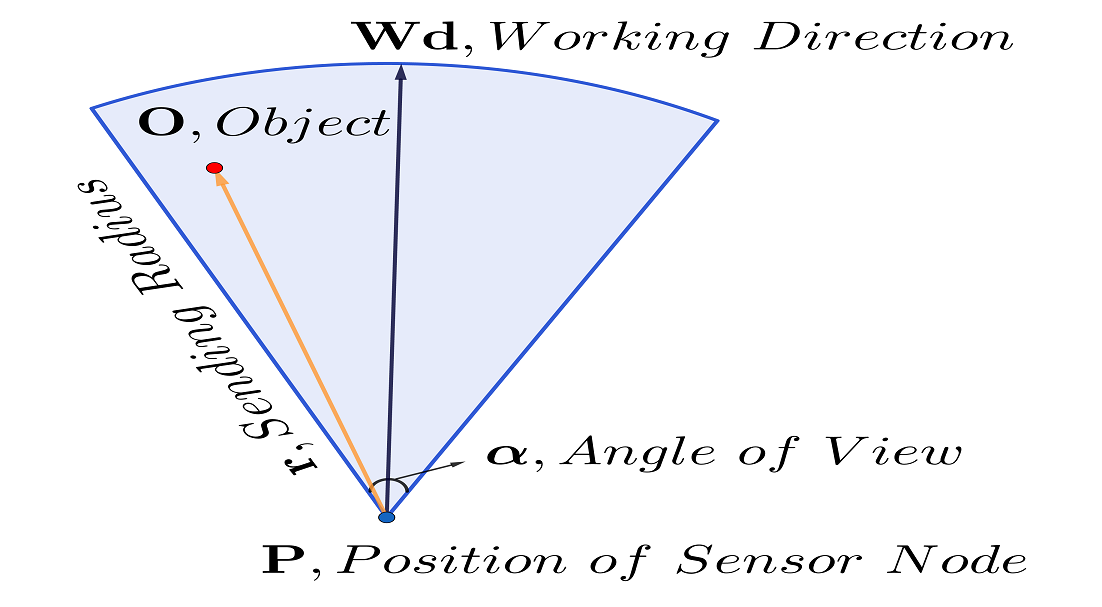
\includegraphics[width=0.4\textwidth]{hinhanh/sensorView}
	% figure caption is below the figure
	\caption{Sensing capability of camera sensor}
	\label{Fig.1_1}      % Give a unique label
\end{figure*}
\begin{equation}
\label{eqfa}
f_a({S_i},O) = \frac{{C{{\left\{ {\cos \left( {\frac{{\angle (\overrightarrow {PO} ,\overrightarrow {Wd}) }}{2}} \right)} \right\}}^\beta }}}{{{{\left[ {d(P,O)} \right]}^\lambda }}}
\end{equation}

where  $A$ is a constant; $\lambda, \ \beta$ are the sensibility attenuation exponents; $d(S_i, O)$ is the distance between $S_i$ and $p$

Closet sensing field intensity

\begin{equation}
\label {eq6}
{S_{\min}(O)} = \{ {S_j} \in S\left| {d({S_j},O) \le d({S_i},O) \ \forall {S_i} \in S, \ i, \ j = \overline {1..N} } \right.\} 
\end{equation}
\begin{equation}
\label{eqic}
I_c(P) = f_a({S_{\min }(O)},P)
\end{equation}

As a result, we devise a more preferable attenuated model assessing the coverage quality of the sensor network toward a point in the field of interest, the model can later be generalized to evaluate the coverage of the sensor network on a line or a closed region.

Considering a point lie in the sensing range of a certain omnidirectional or directional sensor. The sensor $S_i$, the penetration object $P$ with radius $R$ and the considered part $P_\phi$ being positioned at $\phi$ and has length $dl$. Call the distance from $S_i$ to $P_\phi$ as $d_i$, the direction of the sensor compared to the pivot direction as $\phi_i$. Because $R$ is usually inconsiderable compared to $d_i$, we can approximately use $\phi_i$ and $d_i$ as constants with variable $\phi$, the model will be now illustrated as followed.

\begin{figure}[h]
\begin{minipage}{.5\linewidth}
	\centering
	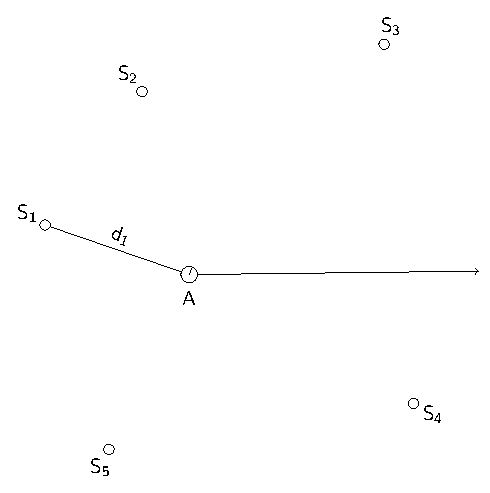
\includegraphics[scale=.75]{groupSensor_Version2.pdf}
\end{minipage}\hfill
\begin{minipage}{.5\linewidth}
	\centering
	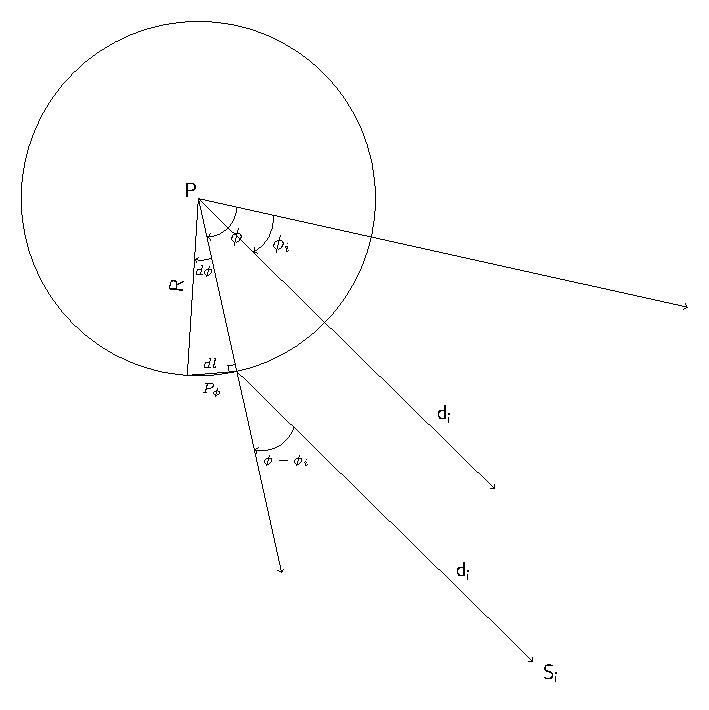
\includegraphics[scale=.6]{exposure.pdf}
\end{minipage}
\end{figure}

Firstly, the coverage value of a sensor to a part is directly affected by the distance between the sensor and the part, and the angle at which the part is viewed by the sensor, this results in the formula:
\begin{equation}
\label{eq1}
\mathsf{max}(\frac{A\cos(\phi - \phi_i)}{Rd_i^\lambda}, 0)dl
\end{equation}


where $\frac{A}{R}$ is a constant coefficient, note that the coverage would fall below 0 if the angle between the direction of the part and the direction of the sensor is larger than $\frac{\pi}{2}$, so we need to set it to 0 in that case. Rewrite $dl = Rd\phi$, we have:
\begin{equation}
\label{eq2}
\mathsf{max}\left\{\frac{A\cos(\phi - \phi_i)}{d_i^\lambda},\ 0\right\}d\phi
\end{equation}

However, it is obviously unnecessary to obtain too much detailed information from the object in the sensing field. This leads to the existence of a constant $E_{\mathsf{max}}$ which corresponds to the maximum necessary coverage on a part with unit length of the circle. To isolate the value from the relative constant $A$, we rewrite it to the Minimum sensing radius $E_{\mathsf{max}} = \frac{A}{d_{\mathsf{min}}^\lambda}$. As a result, our coverage formula could be rewritten as:
\begin{equation}
\label{eq3}
\mathsf{max}\left\{0,\ \mathsf{min}\Big\{\frac{A}{d_{\mathsf{min}}^\lambda}, \frac{Acos(\phi - \phi_1)}{d_i^\lambda}\Big\}\right\}d\phi
\end{equation}

As a result, the coverage on a part $P_\phi$ of several sensors $S_i$, as illustrated above, is the maximum of the coverage on that part of every covered sensor:

\begin{equation}
\label{eq4}
E_\phi(P) = \mathsf{max}\left\{0,\ \mathsf{min}\Big\{\frac{A}{d_{\mathsf{min}}^\lambda},\ \underset{S_i}{\mathsf{max}}\big\{\frac{A\cos(\phi - \phi_i)}{d_i^\lambda}\big\}\Big\}\right\}d\phi
\end{equation}


In short, the coverage on a part of a certain set of sensors is calculated from the largest value of $\displaystyle\frac{Acos(\phi - \phi_1)}{d_i^\lambda}d\phi$ across all sensors, the result then will be a value in the close interval $[0, E_{\mathsf{max}}d\phi]$ that closest to the above computed value. The total coverage on the object is the sum of the coverage on its small parts. Combined with the differentiated form of the formula above, the total coverage would be the integral on all of its parts. As a result, we receive the formula for the total coverage on the object at a certain point in the sensing field:
\begin{equation}
I(P) = \uint\limits_0^{2\pi}{\mathsf{max}\left\{0,\ \mathsf{min}\Big\{\frac{A}{d_{\mathsf{min}}^\lambda}, \ \underset{S_i}{\mathsf{max}}\big(\frac{A\cos(\phi - \phi_i)}{d_i^\lambda}\big)\Big\}\right\}d\phi}
\end{equation}
In conclusion, a new model of coverage is devised which may prove to be exceptionally effective in measuring the coverage efficiency of sensor networks in not only the tradition coverage problem but also in more complex ones such as the problem of $full\hspace{1mm}view$ or multiple view barrier coverage. The new model is proposed with detailed and precise logical progress, successfully adapts the strong points of both the All-Sensor Field Intensity and the Closest-Sensor Field Intensity model \cite{megerian2002exposure}, handling preferably the cooperation of multiple sensors in the network without overrating the repetition of captured information.
%\subsubsection{Coverage of a barrier}	
%\label{bar	rier}

\begin{df}{\itshape($k-\omega$) barrier}\\
	A ($k-\omega$) barrier $B$ is a connected region from the left side to the right side of the monitoring region and satisfies that $B$ is ($k-\omega$) covered.
\end{df}
\begin{df}{\itshape($k-\omega$) barrier coverage}\\
	A region achieves ($k-\omega$) barrier coverage if there exists a ($k-\omega$) barrier in that region.\par
\end{df}

A $(k-\omega)$ barrier (a multiple view barrier) is a region connects the left and right side of the sensing field in which all the points are $(k-\omega)$ covered. Typically, a multiple view barrier is fairly narrow, and penetration objects usually intersect the barrier only at a small part on their paths. As a result, a proper metric to assess the efficiency of the multiple view barrier would be the coverage density of it.

With the same set of sensors considered, in the range of coverage of all elements of that set, the coverage function is always continuous. Since a barrier is consisted of several separated parts each of which is $k-\omega$ covered by a common set of sensors, the coverage density of the barrier can be defined as the quotient of the total coverage in the barrier and the area of that area, with the total coverage being formulated as the integral of the coverage function over the barrier region. Call the barrier region $B$ with area $S_B$, the coverage density over $B$, which is $D_B$ can be formulated as
\begin{equation}
\label{eq5}
I(B) = \iint_B{E(x, y)dxdy}.\frac{1}{S_B}
\end{equation}

